%&pdflatex
\documentclass[final,leqno]{siamltex}
%\documentclass[10pt,onecolumn]{article}
\usepackage[top=2cm,bottom=3cm,left=3.5cm,right=3.5cm]{geometry}
\usepackage[utf8]{inputenc}
\usepackage{amsmath,amssymb,amsfonts,mathrsfs}
\let\proof\relax 
\let\endproof\relax
\usepackage{listings}
\usepackage{array}
\usepackage{mathtools}
\usepackage{dsfont}
\usepackage{graphicx}
\usepackage{pdfpages}
\usepackage[textsize=footnotesize,color=green]{todonotes}
\usepackage{algorithm, algorithmic}
\usepackage{array}
\usepackage{bm}
\usepackage{tikz}
\usepackage{subfigure}
\usepackage[normalem]{ulem}

%\usepackage{lineno}
%\pagewiselinenumbers
%\usepackage{uselinenofix}


\newcommand{\bs}[1]{\boldsymbol{#1}}

\newcommand{\equaldef}{\stackrel{\mathrm{def}}{=}}

\newcommand{\tablab}[1]{\label{tab:#1}}
\newcommand{\tabref}[1]{Table~\ref{tab:#1}}

\newcommand{\theolab}[1]{\label{theo:#1}}
\newcommand{\theoref}[1]{\ref{theo:#1}}
\newcommand{\eqnlab}[1]{\label{eq:#1}}
\newcommand{\eqnref}[1]{\eqref{eq:#1}}
\newcommand{\seclab}[1]{\label{sec:#1}}
\newcommand{\secref}[1]{\ref{sec:#1}}
\newcommand{\lemlab}[1]{\label{lem:#1}}
\newcommand{\lemref}[1]{\ref{lem:#1}}

\newcommand{\mb}[1]{\mathbf{#1}}
\newcommand{\mbb}[1]{\mathbb{#1}}
\newcommand{\mc}[1]{\mathcal{#1}}
\newcommand{\nor}[1]{\left\| #1 \right\|}
\newcommand{\snor}[1]{\left| #1 \right|}
\newcommand{\LRp}[1]{\left( #1 \right)}
\newcommand{\LRs}[1]{\left[ #1 \right]}
\newcommand{\LRa}[1]{\left\langle #1 \right\rangle}
\newcommand{\LRc}[1]{\left\{ #1 \right\}}
\newcommand{\LRb}[1]{\left| #1 \right|}

\newcommand{\tanbui}[2]{\textcolor{blue}{\sout{#1}} \textcolor{red}{#2}}
\newcommand{\Grad} {\ensuremath{\nabla}}
\newcommand{\Div} {\ensuremath{\nabla\cdot}}
\newcommand{\Nel} {\ensuremath{{N^\text{el}}}}
\newcommand{\jump}[1] {\ensuremath{\LRs{\!\left[#1\right]\!}}}
\newcommand{\uh}{\widehat{u}}
\newcommand{\fnh}{\widehat{f}_n}
\renewcommand{\L}{L^2\LRp{\Omega}}
\newcommand{\pO}{\partial\Omega}
\newcommand{\Gh}{\Gamma_h}
\newcommand{\Gm}{\Gamma_{-}}
\newcommand{\Gp}{\Gamma_{+}}
\newcommand{\Go}{\Gamma_0}
\newcommand{\Oh}{\Omega_h}

\newcommand{\eval}[2][\right]{\relax
  \ifx#1\right\relax \left.\fi#2#1\rvert}

\def\etal{{\it et al.~}}

\newcommand{\vect}[1]{\ensuremath\boldsymbol{#1}}
\newcommand{\tensor}[1]{\underline{\vect{#1}}}
\newcommand{\del}{\Delta}
\let\grad\relax
\newcommand{\grad}{\nabla}
\newcommand{\curl}{\grad \times}
\renewcommand{\div}{\grad \cdot}
\newcommand{\ip}[1]{\left\langle #1 \right\rangle}
\newcommand{\eip}[1]{a\left( #1 \right)}
\newcommand{\pd}[2]{\frac{\partial#1}{\partial#2}}
\newcommand{\pdd}[2]{\frac{\partial^2#1}{\partial#2^2}}

\newcommand{\circone}{\ding{192}}
\newcommand{\circtwo}{\ding{193}}
\newcommand{\circthree}{\ding{194}}
\newcommand{\circfour}{\ding{195}}
\newcommand{\circfive}{\ding{196}}

\def\arr#1#2#3#4{\left[
\begin{array}{cc}
#1 & #2\\
#3 & #4\\
\end{array}
\right]}
\def\vecttwo#1#2{\left[
\begin{array}{c}
#1\\
#2\\
\end{array}
\right]}
\def\vectthree#1#2#3{\left[
\begin{array}{c}
#1\\
#2\\
#3\\
\end{array}
\right]}
\def\vectfour#1#2#3#4{\left[
\begin{array}{c}
#1\\
#2\\
#3\\
#4\\
\end{array}
\right]}

%\newtheorem{proposition}{Proposition}
%\newtheorem{corollary}{Corollary}
%\newtheorem{theorem}{Theorem}
%\newtheorem{lemma}{Lemma}

\newcommand{\G} {\Gamma}
\newcommand{\Gin} {\Gamma_{in}}
\newcommand{\Gout} {\Gamma_{out}}
\newcommand{\insub}{{\rm in}}
\newcommand{\outsub}{{\rm out}}

\newtheorem{remark}{Remark}

\title{Primal DPG formulation for convection-diffusion}
\author{}
\date{}
\begin{document}

Our original variational formulation for the convection-diffusion problem is 
\[
b(u,v) = \LRa{\beta_n u,v}_{\Gamma} + \LRp{u,-\beta \grad v} - \epsilon \LRa{\pd{u}{n},v}_{\Gin} + \epsilon\LRp{\Grad u, \Grad v}_{\L} = \LRp{f,v}_{\L} , \quad \forall v \in H^1_\outsub
\]
where 
\begin{align*}
\Gamma_{\rm in}\coloneqq \LRc{x\in \partial \Omega: \beta\cdot\vec{n}(x) < 0}\\
\Gamma_{\rm out}\coloneqq \LRc{x\in \partial \Omega: \beta\cdot\vec{n}(x) > 0}.
\end{align*}
Boundary conditions can be applied in either a strong or weak fashion in this formulation.  

This formulation is derived under the assumption that $v$ is $C_0$ continuous throughout the domain.  However, if we break that continuity and require only that $v\in H^1(K)$ (i.e. in $H^1$ locally), we can derive a different variational formulation.  Integrating by parts, we pick up a boundary term over each element, such that our variational form becomes
\begin{align*}
b\LRp{\LRp{u,\fnh},v} &= \LRa{\beta_n u,v}_{\Gamma} + \LRp{u,-\beta \grad v} - \LRa{\fnh,\jump{v}}_{\Gh^0} - \epsilon \LRa{\pd{u}{n},v}_{\Gamma} + \epsilon\LRp{\Grad u, \Grad v}_{\L} \\
&= \LRp{f,v}_{\L} , \quad \forall v \in H^1_\outsub.
\end{align*}
where we have identified the viscous fluxes $\epsilon\pd{u}{n}$ on the interior skeleton $\Gh^0$ as additional unknowns $\fnh$.  

\section{Interpretation as a nonconforming method for $e$}

The abstract mixed form of the DPG method with $(e,v)\in V$ and $(u,du)\in U$ is given as
\begin{align*}
(e,v)_V + b(u,v) &= l(v)\\
b(\delta u,e) &= 0.
\end{align*}
This is equivalent to a constrained projection/Riesz inversion 
\begin{align*}
(e,v)_V &= l(v), \quad (e,v) \in V\cap{\rm null}(B^T)
\end{align*}
where $B: U\rightarrow V'$ is defined through $\LRa{Bu,v} = b(u,v)$.  

If we choose a broken test space $\LRc{ v\in \L, \left.v\right|_K \in V(K)}$, we can enforce continuity between elements by penalizing the jumps of $e$ using a Lagrange multiplier method
\begin{align*}
(e,v)_V + b(u,v) + \LRa{\lambda, \jump{v}}_{\Gh}&= l(v)\\
b(\delta u,e) + \LRa{\delta \lambda, \jump{e}}_{\Gh} &= 0.
\end{align*}
where $\lambda$ is a function with support only on $\Gh$, the mesh skeleton.  This is equivalent to the mixed DPG formulation under the bilinear form $b_h((u,\fnh),v) \coloneqq b(u,v) + \LRa{\fnh, \jump{v}}_{\Gh}$, with additional trace unknowns $\fnh$.  The advantage of this formulation is that the degrees of freedom for $e$ can be condensed out and eliminated, leaving a positive definite system for $u$ and $\fnh$, and is equivalent to locally computing optimal test functions.  

\section{Initial numerical results}

Both the primal and original $C_0$ mixed DPG methods for convection-diffusion display optimal rates, and display nearly identical $L^2$ errors on the same mesh.  Below are comparisons of $L^2$-errors under uniform refinement.  The flux variable $\fnh$ is taken to be the trace of Raviart-Thomas elements of equal order to the field variables $u$ (this can be relaxed to be $p-1$, where $p$ is the order of $u$).  

\begin{figure}[!h]
\centering
\subfigure[Primal DPG]{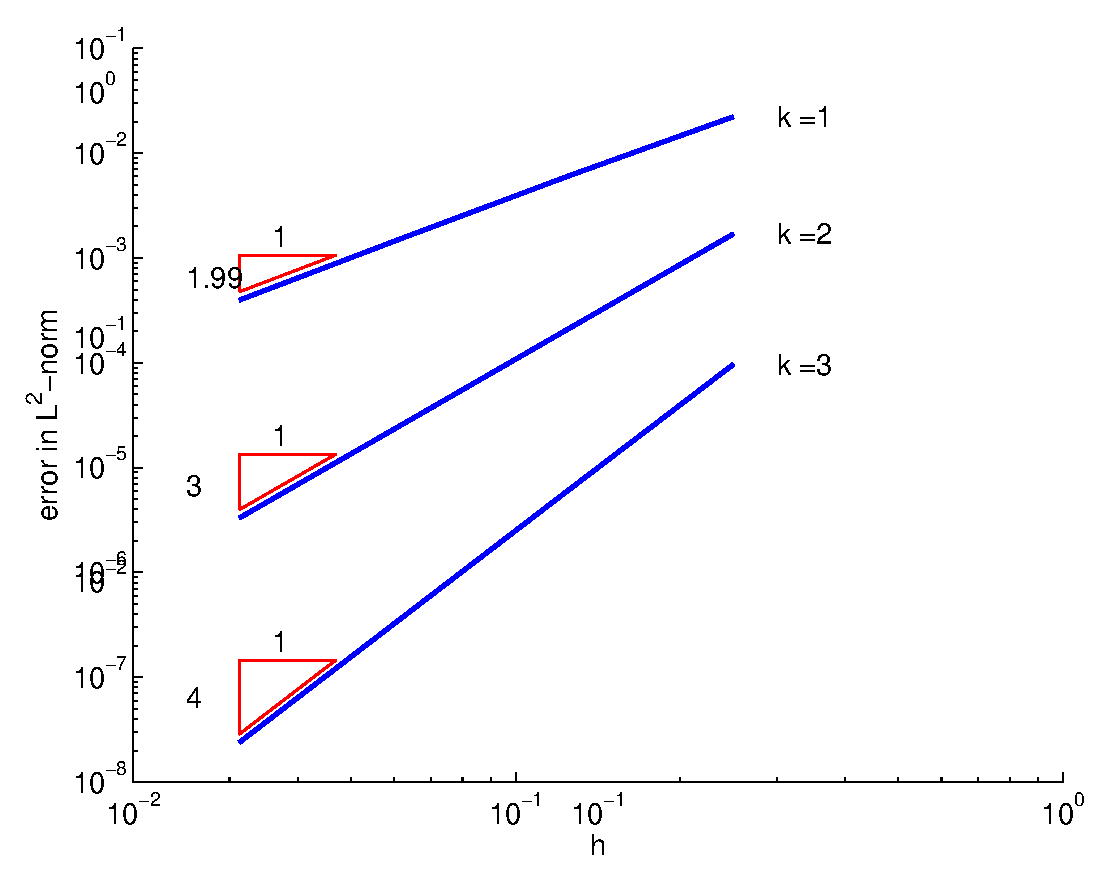
\includegraphics[width = .49\textwidth]{figs/matlab/primal_eps1e0_h.eps}}
\subfigure[Mixed $C_0$ DPG]{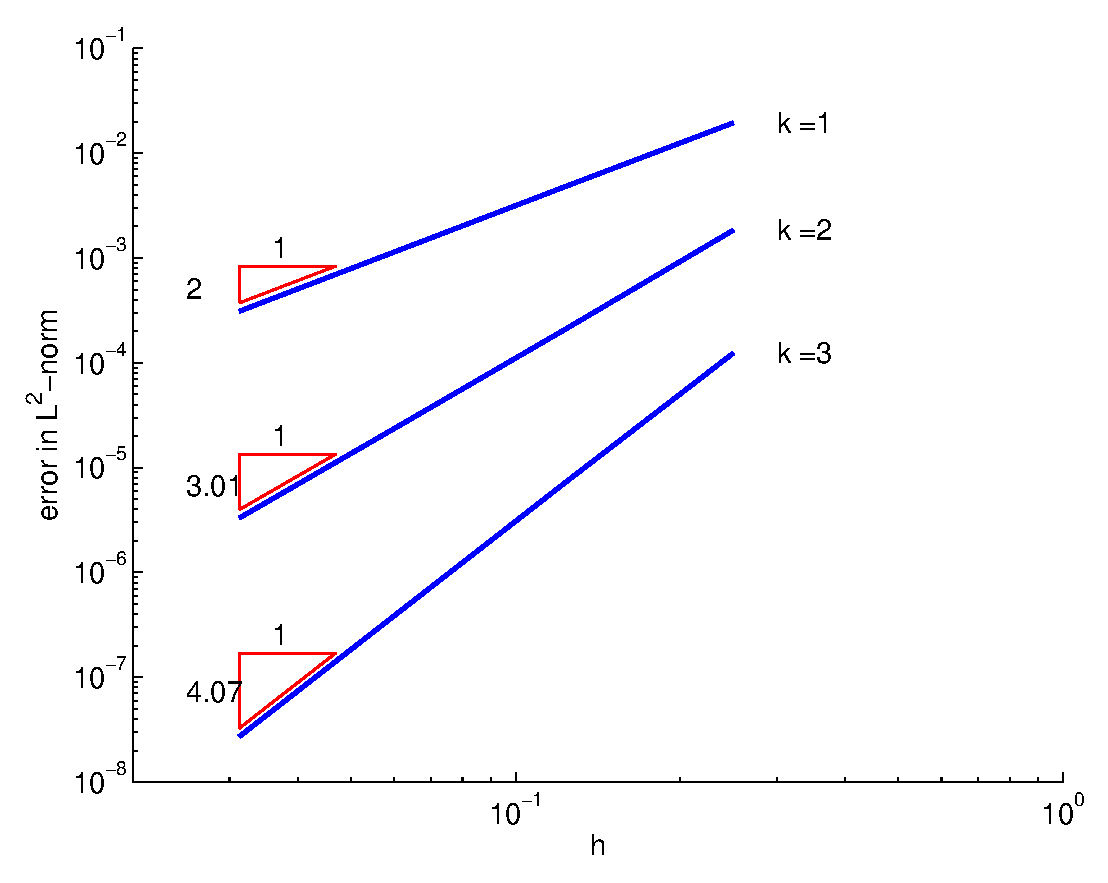
\includegraphics[width = .49\textwidth]{figs/matlab/mixed_eps1e0_h.eps}}
%\subfigure[$\epsilon = 1e-4$]{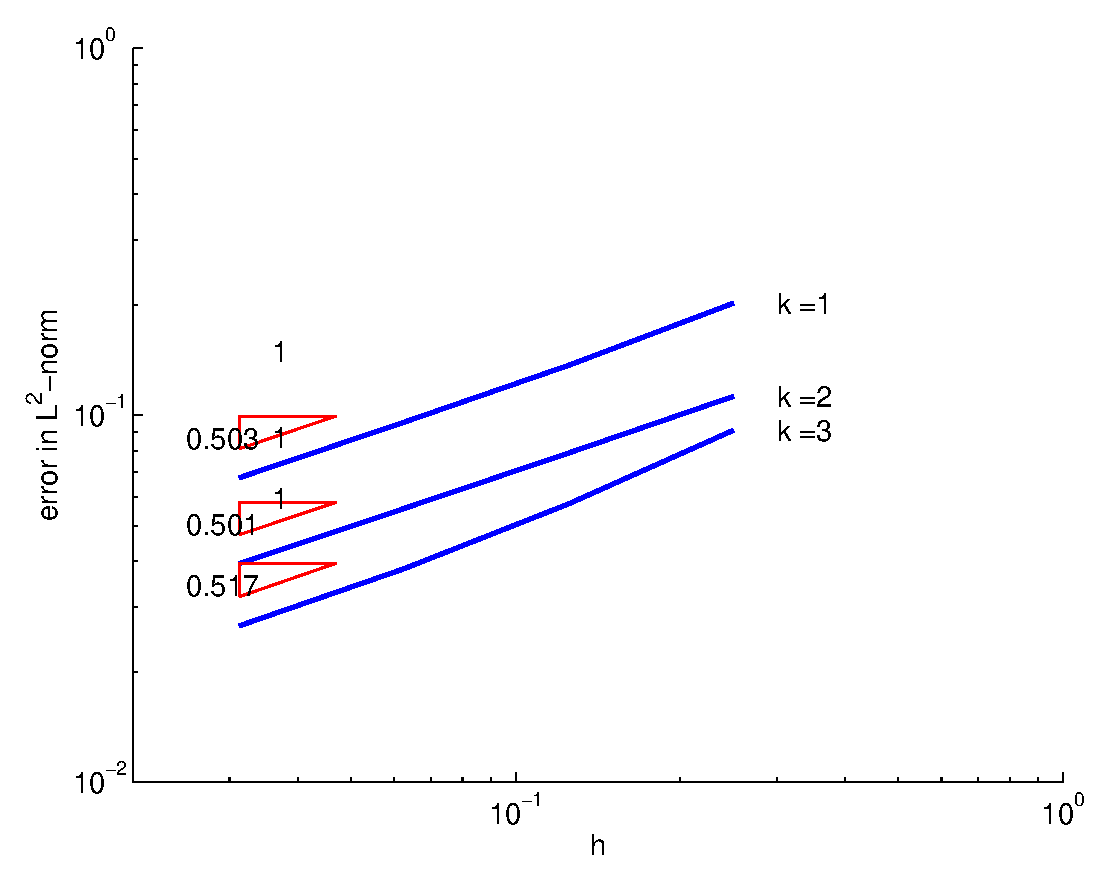
\includegraphics[width = .49\textwidth]{figs/matlab/primal_eps1e4_h.eps}}
\caption{Rates for primal and $C_0$ mixed DPG method for $\epsilon = 1.0$.}
\label{fig:comparison1D}
\end{figure}

\begin{figure}[!h]
\centering
\subfigure[Primal DPG]{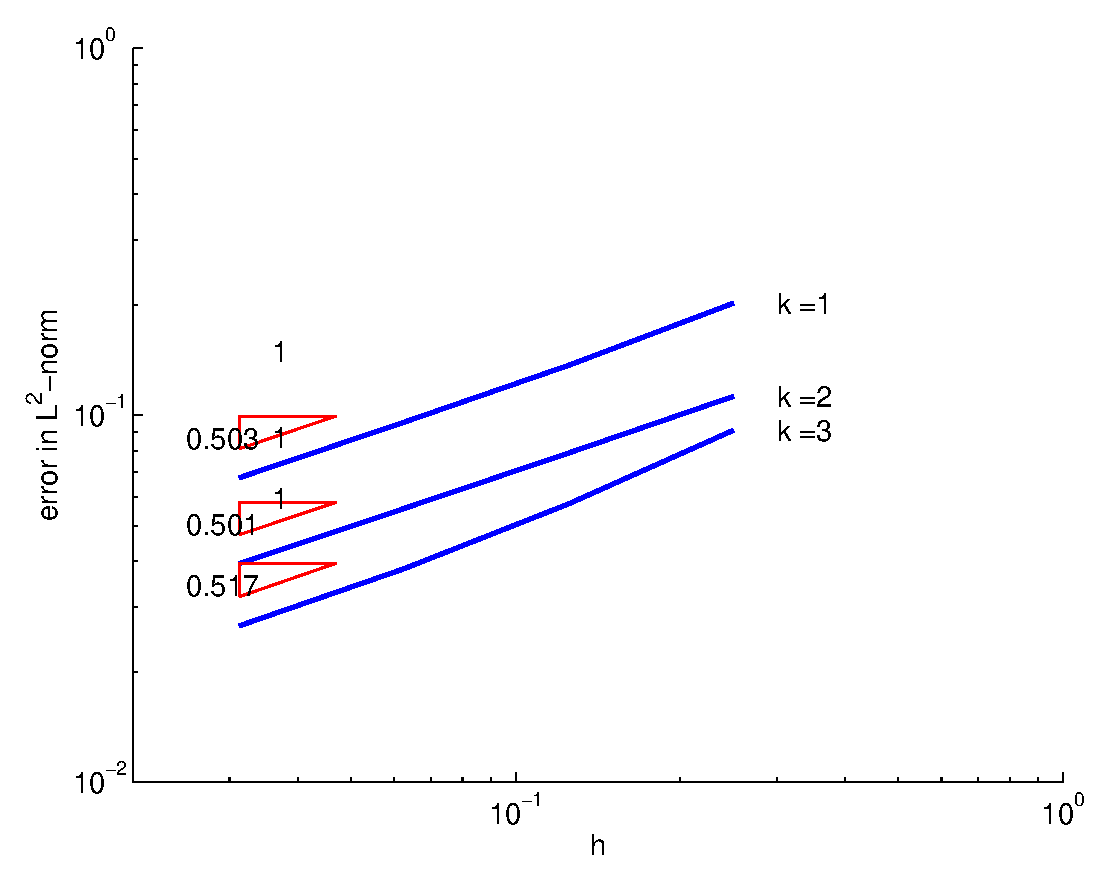
\includegraphics[width = .49\textwidth]{figs/matlab/primal_eps1e4_h.eps}}
\subfigure[Mixed $C_0$ DPG]{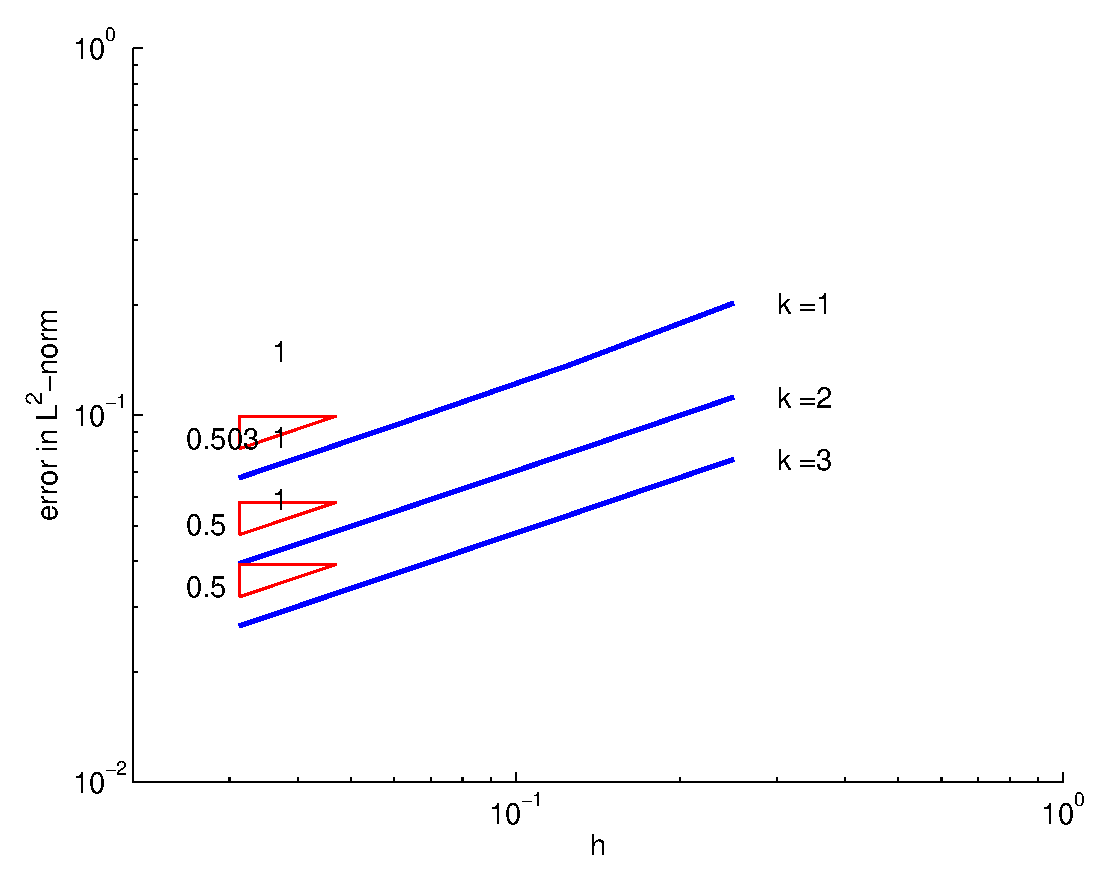
\includegraphics[width=.49\textwidth]{figs/matlab/mixed_eps1e4_h.eps}}
\caption{Rates for primal and $C_0$ mixed DPG methods for $\epsilon = 1e-4$}
\end{figure}

\end{document}